% Copyright (c) 2014,2016 Casper Ti. Vector
% Public domain.

\chapter{利用CNN分辨NLDBD事件和背景事件}
\label{chapter:cnn}

\section{测试}
\subsection{读出平面的结构}

PandaXIII设计使用了41个Microbulk Micromegas读出板来构建读出平面,每个MM(Microbulk Micromegas)板的尺寸为20厘米x20厘米,按照图\ref{fig:mms}所示的形状排列组成。

\begin{figure}[tbh]
    \centering
    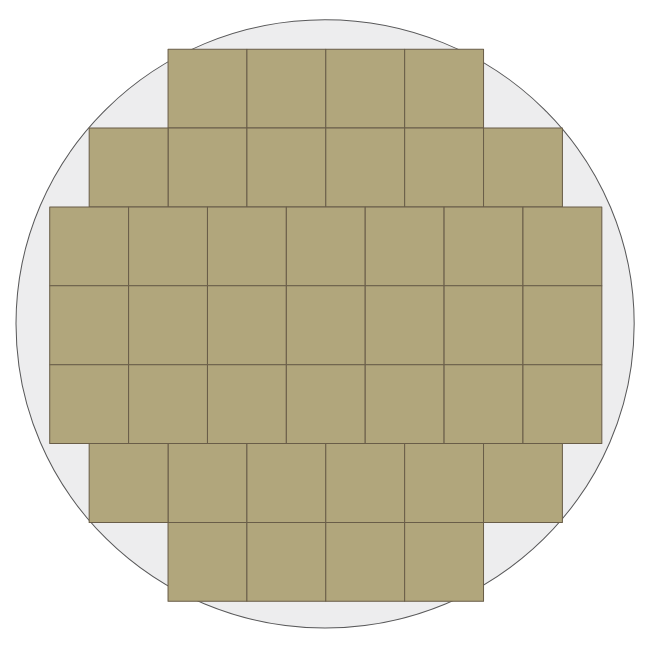
\includegraphics[width=0.4\columnwidth]{pic/fig8.png}
    \caption{41个MM板组合探测器读出平面排放示意图,按照4,6,7,7,7,6,4层叠放置。}
    \label{fig:mms}
\end{figure}

需要注意的是,在背景模拟过程中我们并没有考虑读出平面对于背景信号的影响,而是在探测器效率以及后续的使用CNN分辨事件

% vim:ts=4:sw=4
